%
% Sample conclusion of your thesis
%

\chapter{Masking the Ring-LWE Encryption Scheme I}
Since most side-channel attacks focus on the decryption operation, this section will present an attempt to masking the decryption function of the \textit{LPR} Ring-LWE encryption scheme. This masking approach was originally proposed in \cite{maskedRing}, for more details we would refer you to that paper.

\section{Implementation}
W will start by giving the reader an overview of the general setup, before going into more detail about the masked decoding algorithms. We will make strong use of the \textit{Number Theoretic Transform} (NTT) in this chapter. We recall, that our notation for polynomials in the NTT domain is \(\tilde{\textbf{f}}\). The NTT operation itself will be denoted as \(\textsc{NTT}(.)\), while its inverse operation will be written as \(\textsc{INTT}(.)\). We want to stress, that \(\textsc{NTT}(.)\) and \(\textsc{INTT}(.)\) are linear operations, as we will use this characteristic for our blinding technique.

\subsection{Overview}
This Subsection will cover a concise overview of the blinding technique proposed in \cite{maskedRing}.  For the sake of simplicity, the intermediate \(m_{enc}\) will be referred to as \(a\) in the following.\\
We start by splitting the secret key \(\textbf{s}\) into two shares \(\textbf{s}',\textbf{s}'' \in R_q\) such that \(\textbf{s}=\textbf{s}'+\textbf{s}''\). Therefore we choose all coefficients of \(\textbf{s}'\) uniformly at random and calculate \(\textbf{s}''=\textbf{s}-\textbf{s}'\). In the NTT domain it follows that \(\tilde{\textbf{s}}=\tilde{\textbf{s}}'+\tilde{\textbf{s}}''\). Due to the linearity of \(\textsc{INTT}(.)\) and the multiplication, we can compute \(\textbf{a}\) as:
\begin{equation}
	\textbf{a}=\textsc{INTT}(\tilde{\textbf{s}} \cdot \tilde{\textbf{c}}_1+\tilde{\textbf{c}}_2)=\textsc{INTT}(\tilde{\textbf{s}}' \cdot \tilde{\textbf{c}}_1+\tilde{\textbf{c}}_2)+\textsc{INTT}(\tilde{\textbf{s}}'' \cdot \tilde{\textbf{c}}_1)
\end{equation}
This enables us to split the whole equation into two branches, calculating \(\textbf{m}'_{enc}\) and \(\textbf{m}''_{enc}\) in the following way:
\begin{equation}
	\textbf{a}'=\textsc{INTT}(\tilde{\textbf{s}}' \cdot \tilde{\textbf{c}}_1+\tilde{\textbf{c}}_2),\:\textbf{a}''=\textsc{INTT}(\tilde{\textbf{s}}'' \cdot \tilde{\textbf{c}}_1)
\end{equation}
Those computations can be done on a arithmetic processor without any protection against side-channel attacks like \textit{DPA}, as both branches are totally independent of our secret key \(\textbf{s}\).\\
However, the \(\textsc{Decode}(a_{i})\) function in the decryption stage of the \textit{LPR} scheme is non-linear and cannot easily be split into two parts. For this reason, we will present a masked decoder in the next Subsection, that takes \(\textbf{a}'\) and \(\textbf{a}''\) as inputs to compute two shares \(\textbf{m}'\), \(\textbf{m}''\) of the decoded message \(\textbf{m}\) in a fairly efficient way.

\subsection{Masked Decoder}
This Section briefly describes a probabilistic masked decoder. We recall, that the \(i\)-th element of \(\textit{a}\) is called \(a_i\) and the shares \((a'_i,a''_i)\) of such an element are choosen in a way, that \(a'_i + a''_i = a_i\) (mod \(q\)). To keep it simple, we will refer to an arbitrary \(a_i\) as \(a\), the same follows for it's shares.\\
For our masked decoder, we do not need to know the exact values of \(a'\) and \(a''\) to compute \(\textsc{Decode}(a)\). The following example will help us to lay down some rules for the decoder: Given \((a', a'')\) with \(0 < a' < q/4\) and \(q/4 < a'' < q/2\). Then know that for \(a=a'+a''\) it follows, that \(q/4 < a < 3q/4\) and therefore \(\textsc{Decode}(a)=1\). We only need to know the most significant bits of \(a'\) and \(a''\) to determine, which values they are bounded by.
\begin{figure}
	\centering
	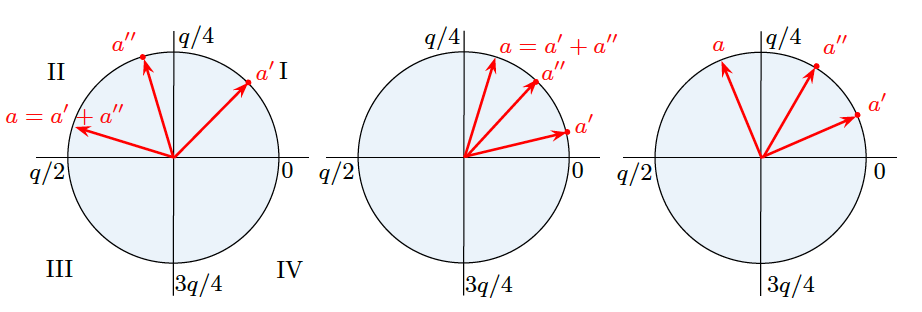
\includegraphics[width=\textwidth]{maskedDecoder_1.png}
	\caption{The basic idea of our masked decoder. The circle represents elements in \(\mathbb{Z}_q\). The first case shown allows us to conclude \(\textsc{Decode}(a)=1\), while we cannot make any guesses about the last two ones. \cite{maskedRing}}
	\label{maskedDecoder_1}
\end{figure}
\\Figure \ref{maskedDecoder_1} shows our example from above on the left. We can use this knowlegde to state a total of four rules, the first of whom is taken from our example:
\begin{itemize}
\item \(0 < a' < q/4\), \(q/4 < a'' < q/2\) \(\implies\) \(a \in (q/4,3q/4)\) \(\implies\) \(\textsc{Decode}(a)=1\)
\item \(q/2 < a' < 3q/4\), \(3q/4 < a'' < q\) \(\implies\) \(a \in (q/4,3q/4)\) \(\implies\) \(\textsc{Decode}(a)=1\)
\item \(q/4 < a' < q/2\), \(q/2 < a'' < 3q/4\) \(\implies\) \(a \in (0,q/4) \cup (3q/4,q)\) \(\implies\) \(\textsc{Decode}(a)=0\)
\item \(3q/4 < a' < q\), \(0 < a'' < q/4\) \(\implies\) \(a \in (0,q/4) \cup (3q/4,q)\) \(\implies\) \(\textsc{Decode}(a)=0\)
\end{itemize}
With swapping \(a'\) and \(a''\) in the above rules, one can obtain another four rules. From the rules it follows, that we only need to know the quadrant of each \(a'\) an \(a''\) to infer the output of \(\textsc{Decode}(a)\). However, this does not work for all cases, as Figure \ref{maskedDecoder_1} shows. We can actually only apply those rules in half of the possible cases.\\
So, what happens if our \((a', a'')\) does not match any rule? We simply need to refresh the splitting by computing \(a' = a' + \Delta_1\) and \(a'' = a'' - \Delta_1\) with \(\Delta_i \in \mathbb{Z}_q\). From \((a' + \Delta_1) + (a'' - \Delta_1) = a' + a'' = a\) it follow, that \(a\) stays unchanged by that refresh. Now that we have a fresh pair \((a',a'')\), we can again try to apply our rules from above. This process can be repeated until all shares have been decoded. Note, that a new \(\Delta_i\) should be choosen for each iteration. About half of the \(a',a''\) are decoded per iteration, so that the amount of decoded shares rises exponentially with the number of iterations. The authors of \cite{maskedRing} propose a number of \(N = 16\) iterations for a satisfactory result.
\begin{figure}
	\centering
	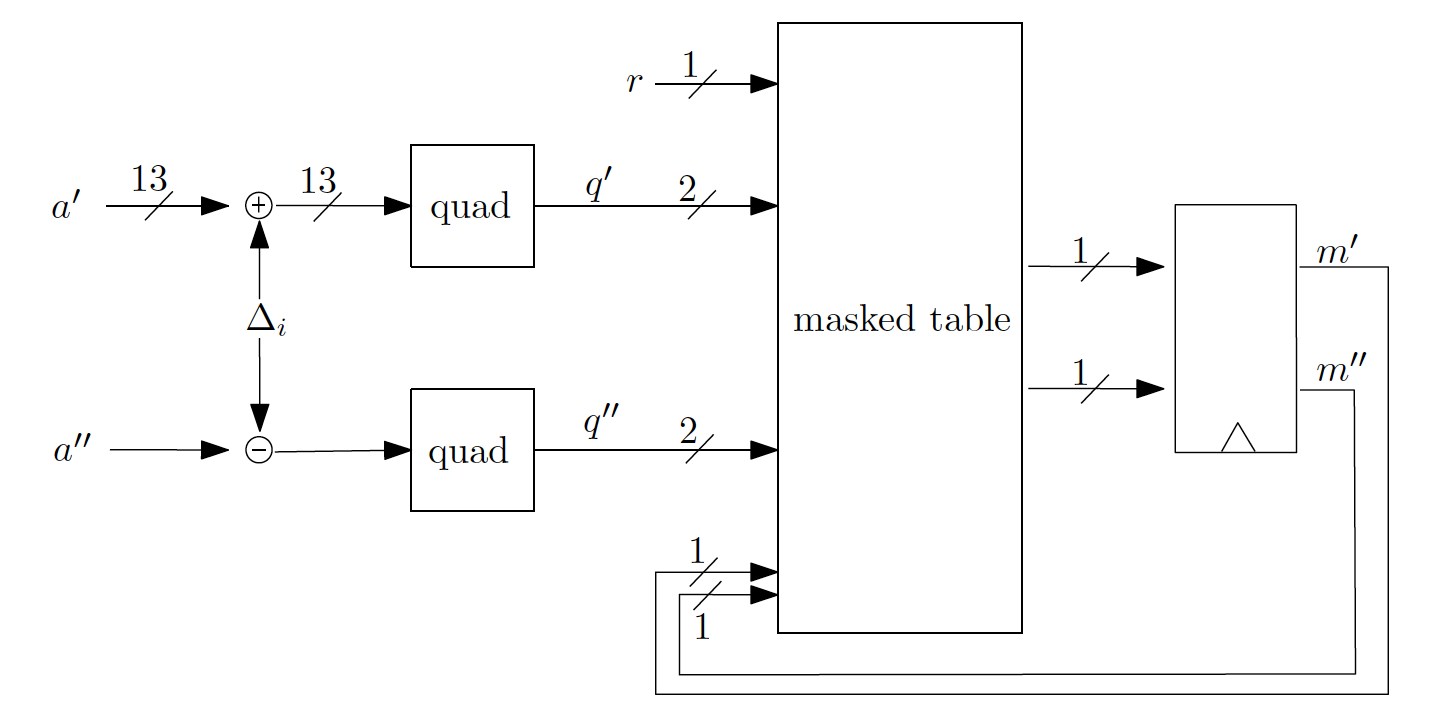
\includegraphics[width=0.7\textwidth]{maskedDecoder_2.png}
	\caption{Hardware implementation of the masked decoder. \cite{maskedRing}}
	\label{maskedDecoder_2}
\end{figure}
\\A possible hardware implementation of such a masked decoder is shown in Figure \ref{maskedDecoder_2}. The refreshing step is depicted on the left, using a different \(\Delta_i\) in each iteration. The quadrant function used in the next step simply takes a refreshed share \(a'\) or \(a''\) as an input and outputs two bits depending on the quadrant that the share belongs to. Next, a masked table is used to check the two bits against the rules we described above. Finally, the masked table function returns two one bit shares of the decoded message \(\textit{m}\). In our implementation the masked takes additional inputs, like a random bit \(r\) and the output of the last iteration \((m_{i-1}',m_{i-1}'')\). For more details on the masked table lookup, we would like to refer you to the paper of Oscar Reparaz et. al. \cite{maskedRing}.

%\subsection{Masked Table Lookup}
%Wenn noch Text fehlt, wird das hier eingefügt

\section{Evaluation}